\lecture{15}{Towards Foundation Models for Knowledge Graphs}{Thursday, November 12, 2026}\label{ch:lec15}

\providecommand{\mE}{\mathbf{E}}

% Local TikZ styles (prefix lec15)
\tikzset{
  lec15ent/.style={circle, fill=RoyalBlue, minimum size=2.6mm, inner sep=0pt},
  lec15nm/.style={font=\scriptsize\sffamily, inner sep=1.5pt},
  lec15lbl/.style={font=\tiny\sffamily, fill=white, inner sep=0.6pt},
  lec15e/.style={thick, -{Stealth[length=1.5mm]}},
  lec15born/.style={lec15e, BrickRed},
  lec15act/.style={lec15e, ForestGreen},
  lec15prof/.style={lec15e, Goldenrod},
  lec15dir/.style={lec15e, black},
  lec15co/.style={lec15e, RoyalBlue!80!black},
  lec15rel/.style={circle, fill=RoyalBlue, minimum size=3.6mm, inner sep=0pt},
  lec15w/.style={font=\scriptsize\sffamily, fill=white, inner sep=1pt},
  lec15rg/.style={thick, RoyalBlue!80!black, {Stealth[length=1.6mm]}-{Stealth[length=1.6mm]}},
  lec15blk/.style={draw, rounded corners=2pt, thick, fill=black!4, align=center,
                   font=\scriptsize\sffamily, text width=21mm, minimum height=10mm,
                   inner sep=2pt},
  lec15lw/.style={line width=2.2pt, RoyalBlue!70!black, -{Triangle[length=2.6mm, width=4.4mm]}},
  lec15usr/.style={circle, draw=black!70, thick, fill=Peach!40, minimum size=5mm,
                   inner sep=0pt, font=\tiny\sffamily},
  lec15itm/.style={rectangle, draw=black!70, thick, fill=black!8, minimum size=5mm,
                   inner sep=1pt, font=\tiny\sffamily},
  lec15qry/.style={rectangle, rounded corners=1.5pt, draw=black!70, thick, fill=white,
                   minimum width=13mm, minimum height=4.6mm, inner sep=1pt,
                   font=\tiny\sffamily},
  lec15search/.style={thick, densely dashed, ForestGreen!70},
  lec15click/.style={thick, densely dashed, BrickRed!70},
  lec15guide/.style={thick, densely dashed, Purple!60},
}

\textbf{Outline.} Foundation models across domains $\to$ graph foundation models and the
goal of a foundation model for KGs $\to$ KGs vs natural language $\to$ transductive link
prediction (shallow KG embeddings and their limits) $\to$ inductive link prediction
(heterogeneous GNNs, RGCN) $\to$ inductive link prediction for new entity \emph{and}
relation types $\to$ InGram (relation graph, relation- and entity-level message passing,
link-prediction head, experiments).

% ---------------------------------------------------------------------
\section{Foundation models}\label{sec:lec15-fm}

\subsection{Foundation models across domains}\label{sec:lec15-domains}
\slides{3--8}

\begin{itemize}
  \item \textbf{Large language models} -- \emph{from large-scale pretraining to adaptive
    reasoning}: (01) \textbf{Pretrain}: learn general language representations $\to$
    (02) \textbf{Adapt}: follow instructions and use contextual examples $\to$ (03)
    \textbf{Reason}: use post-training and test-time computation.
    \begin{itemize}
      \item \textbf{DeepSeek-R1} (Guo et al., Nature 2025): RL encourages
        self-reflection, verification and strategy adaptation during reasoning.
      \item \textbf{Qwen3} (Yang et al., arXiv 2025): one model family supports fast
        non-thinking and more compute-intensive thinking modes.
    \end{itemize}
\end{itemize}
\begin{keyidea}[slide 4]
  A pretrained model supports many tasks without training a separate model for each.
\end{keyidea}
\begin{itemize}
  \item \textbf{Relational foundation models} (RT also in \cref{ch:lec14}) --
    \emph{pretrain on linked tables $\to$ transfer across schemas and tasks}:
    relational databases (Commerce: Users $\cdot$ Orders $\cdot$ Items; Finance:
    Accounts $\cdot$ Transactions; Healthcare: Patients $\cdot$ Visits) $\to$
    \textbf{Relational Transformer} (schema-aware tokens + relational attention) $\to$
    predictions (classification: fraud/churn; regression: demand/revenue; forecasting:
    patient/temporal risk).
    \begin{itemize}
      \item \textbf{RT} (Ranjan et al., ICLR 2026): zero-shot transfer to unseen
        databases. \textbf{RT-J} (Ranjan et al., NeurIPS 2026): few-shot, in-context
        prediction.
    \end{itemize}
  \item \textbf{Biology} -- \emph{from molecular sequences to structures and biological
    design}:
    \begin{itemize}
      \item \textbf{ESM3} (Science 2025), proteins: generate conditioned on sequence,
        structure \& function.
      \item \textbf{AlphaFold 3} (Nature 2024), biomolecular complexes: predict joint 3D
        structures of proteins, DNA/RNA \& ligands.
      \item \textbf{Evo 2} (Nature 2026), genomes: model long DNA sequences across
        domains of life.
      \item \textbf{The modality determines the input representation, training objective
        and downstream tasks.}
    \end{itemize}
  \item \textbf{Cell biology} -- \emph{representing a cell from its gene-expression
    profile}: \textbf{Universal Cell Embedding (UCE)} (Rosen et al., Nature 2026; also
    scGPT, Cui et al., Nature Methods 2024).
    \begin{itemize}
      \item Input: single-cell RNA expression. Encoder: sampled gene tokens +
        transformer. Output: reusable cell embedding.
      \item Figure: genes $G_1,\dots,G_8$ of a single cell; genes with expression $>0$
        are sampled by expression and sorted by genomic location (Chr.\ A, Chr.\ B) into
        the transformer input (cell representation); gene tokens are represented using
        protein language models.
    \end{itemize}
  \item \textbf{Medicine} -- \emph{medical images + language $\to$ reusable clinical
    capabilities}: medical images, clinical text, task prompts $\to$ medical
    vision-language foundation model $\to$ diagnosis \& QA, visual grounding, clinical
    explanation.
    \begin{itemize}
      \item \textbf{MedGemma} (Nature Medicine 2026): medical text and multi-imaging
        understanding. \textbf{EVLF-FM} (Bai et al., Nature Medicine 2026): diagnosis,
        grounding and explanations.
    \end{itemize}
\end{itemize}

\subsection{What is a foundation model?}\label{sec:lec15-def}
\slides{9--10}

\begin{definition}[Foundation model, slide 9]\label{def:lec15-fm}
  A \term{foundation model} is a machine learning model trained on large-scale, diverse
  data, typically using self-supervised learning, that learns general-purpose
  representations and can be adapted to a wide range of downstream tasks. Three key
  characteristics:
  \begin{enumerate}[label=\arabic*.]
    \item \textbf{Large-scale pretraining:} the model learns from substantial amounts of
      data, often without requiring manually annotated labels.
    \item \textbf{Transferability:} the learned representations or capabilities
      generalize across multiple tasks rather than being optimized for a single task.
    \item \textbf{Adaptability:} the model can be adapted to downstream tasks through
      fine-tuning, prompting, in-context learning, or task-specific prediction heads.
  \end{enumerate}
\end{definition}

\textbf{Foundation model characteristics} (slide~10):
\begin{itemize}
  \item Foundation models are \textbf{pretrained architectures}; modern AI trains
    \textbf{very large models with a huge amount of data}.
  \item \textbf{Foundation models can be used as zero-shot or few-shot learners.}
  \item \textbf{They generalize to new entities that have not been observed during
    training.}
\end{itemize}

\subsection{Graph foundation models}\label{sec:lec15-gfm}
\slides{11--13}

\begin{itemize}
  \item \textbf{Challenges:} \textbf{multiple types of graphs} (figures: a social network
    of people; the KG landscape -- Wikidata, Freebase, NELL, DBpedia, YAGO, ConceptNet,
    OpenIE, Cyc, GeoNames, GDelt, PROSPERA, WordNet, Metaweb, Knowledge Vault; molecules
    labelled non-toxic/approved, toxic/not approved, toxic/approved) and
    \textbf{multiple types of tasks}.
  \item \textbf{Recap: PRODIGY} (\cref{ch:lec14}): \textbf{unified framework to learn
    graph tasks of multiple levels}; \textbf{agnostic of the graph type}. Pipeline:
    pretraining data/graph $\to$ data gen $\to$ task graph over data graphs
    $\mathcal{G}^d$ (prompt examples $\mathcal{S}$, queries $\mathcal{Q}$) $\to$ model
    $\to$ optimize loss.
  \item \textbf{Towards foundation models for KGs} -- the goal of this lecture:
    \begin{itemize}
      \item build a model that \textbf{learns embeddings} for \textbf{entities} and
        \textbf{relations} of \textbf{any KG};
      \item the model will be trained in an \textbf{unsupervised fashion};
      \item the model will \textbf{transfer knowledge} between different KGs;
      \item we \textbf{will not discuss} scalability of the training data and the model.
    \end{itemize}
\end{itemize}

% ---------------------------------------------------------------------
\section{Knowledge graphs}\label{sec:lec15-kg}

\subsection{KG representation and examples}\label{sec:lec15-kgrep}
\slides{14--18}

\begin{itemize}
  \item \textbf{KG representation} as in \cref{ch:lec10}: edges are \term{triples}
    $(h,r,t)$ (head $h$ has relation $r$ with tail $t$); entities and relations get
    \textbf{shallow embeddings} in $\R^k$ (\textbf{no GNN}); the embedding of $(h,r)$
    should be close to the embedding of $t$; score $f_r(h,t)$ high if $(h,r,t)$ exists,
    else low.
  \item \textbf{Examples} as in \cref{ch:lec10}: bio KG (node types drug, disease,
    adverse event, protein, pathways; relations has\_func, causes, assoc, treats, is\_a)
    and bibliographic network (paper, title, author, conference, year; pubWhere,
    pubYear, hasTitle, hasAuthor, cite).
  \item \textbf{E-commerce graph} as in \cref{ch:lec09}: node types User, Item, Query,
    Location, \dots; edge types Purchase, Visit, Guide, Search, \dots; different node
    types' feature spaces can be different (figure: users -- items -- queries Shoes,
    Ladies Bag, Hand Bag, with Search / Click / Guide edges).
\end{itemize}

\subsection{KG vs natural language}\label{sec:lec15-kgnl}
\slides{19--21}

Example (e-commerce graph), natural language: ``User searches for shoes, User buys
hand-bag'' (\cref{tab:lec15-kgnl}).

\begin{table}[htbp]
  \centering\small
  \caption{KG vs natural language (slides~19--21).}
  \label{tab:lec15-kgnl}
  \renewcommand{\arraystretch}{1.2}
  \begin{tabularx}{\textwidth}{@{}l>{\raggedright\arraybackslash}X>{\raggedright\arraybackslash}X@{}}
    \toprule
     & Natural language & Knowledge graph\\
    \midrule
    Vocabulary & All entities are words or tokens of the same type (boxed: User,
      searches, shoes, User, buys, hand-bag) $\Rightarrow$ \textbf{homogeneous
      vocabulary}
      & User, shoes, hand-bag $\to$ \textbf{entities}; searches, buys $\to$
      \textbf{relations} $\Rightarrow$ \textbf{two modalities, heterogeneous
      vocabulary}\\
    Structure & \textbf{Tokens are connected sequentially}
      & \textbf{Entities have an underlying complex graph structure}\\
    \bottomrule
  \end{tabularx}
\end{table}

\subsection{Towards foundation models for KGs: the recipe}\label{sec:lec15-recipe}
\slides{22}

\begin{keyidea}[slide 22]
  \begin{itemize}
    \item Build a model that \textbf{learns embeddings} for \textbf{entities} and
      \textbf{relations} of \textbf{any KG} $\Rightarrow$ \textbf{double equivariant
      architectures}.
    \item Process the graph structure between entities $\Rightarrow$ \textbf{use Graph
      Neural Networks}.
    \item Find a canonical task for unsupervised training $\Rightarrow$
      \textbf{Knowledge Graph Completion}.
  \end{itemize}
\end{keyidea}

% ---------------------------------------------------------------------
\section{Transductive link prediction}\label{sec:lec15-trans}

\subsection{Recap: KG completion and shallow KG embeddings}\label{sec:lec15-recap}
\slides{23--26}

All as in \cref{ch:lec10}:
\begin{itemize}
  \item \textbf{KG completion:} given an enormous KG, can we complete the KG? For a given
    (\textbf{head}, \textbf{relation}), we predict missing \textbf{tails}; e.g.\ predict
    the tail ``Science Fiction'' for (``J.K.\ Rowling'', ``genre'').
  \item \textbf{Shallow encoding:} encoder is just an embedding-lookup; embedding matrix
    $\mZ$, one column per node, rows = dimension/size of embeddings.
  \item \textbf{KG embedding models:} TransE, TransR, DistMult, ComplEx, RotatE (written
    ``RotateE'') -- scores, embedding spaces and relation patterns (Sym., Antisym.,
    Inv., Compos., 1-to-N) as in the \cref{ch:lec10} table (here TransR is written with
    $\vh,\mathbf{t}\in\R^k$, $\vr\in\R^d$, $\mM_r\in\R^{d\times k}$).
\end{itemize}

\subsection{Limitations of KG embedding methods}\label{sec:lec15-limits}
\slides{27--29}

\begin{itemize}
  \item \textbf{KG embedding methods} (slide~27):
    \begin{itemize}
      \item \textbf{Structure agnostic shallow encoders learn embeddings} for
        \textbf{entities} and \textbf{relations}: the entity and relation embeddings
        \textbf{are the trainable weights}.
      \item The structure of the KG is utilized \textbf{in the loss function}.
      \item KG embedding methods can \textbf{only be used on a single KG}: they
        \textbf{cannot transfer knowledge between KGs}.
    \end{itemize}
  \item \textbf{New entities in bio KGs} (slide~28, the bio KG of slide~16): \textbf{what
    if a new drug comes in?} $\Rightarrow$ \textbf{need to retrain the shallow
    encoder}.
  \item \textbf{Generalize across similar KGs} (slide~29): what if I want to
    \textbf{transfer knowledge from one KG to another}? \textbf{The KGs have the same
    relations} (\cref{fig:lec15-similar}).
\end{itemize}

\begin{figure}[htbp]
  \centering
  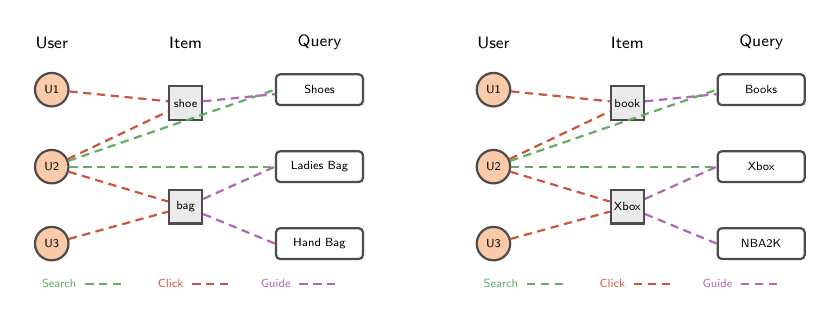
\begin{tikzpicture}[scale=0.85, transform shape]
    \foreach \dx/\ia/\ib/\qa/\qb/\qc in {0/shoe/bag/Shoes/Ladies Bag/Hand Bag,
                                         6.6/book/Xbox/Books/Xbox/NBA2K} {
      \begin{scope}[xshift=\dx cm]
        \node[font=\scriptsize\sffamily] at (0,3.0) {User};
        \node[font=\scriptsize\sffamily] at (2.0,3.0) {Item};
        \node[font=\scriptsize\sffamily] at (4.0,3.0) {Query};
        \node[lec15usr] (u1) at (0,2.3) {U1};
        \node[lec15usr] (u2) at (0,1.15) {U2};
        \node[lec15usr] (u3) at (0,0) {U3};
        \node[lec15itm] (i1) at (2.0,2.1) {\ia};
        \node[lec15itm] (i2) at (2.0,0.55) {\ib};
        \node[lec15qry] (q1) at (4.0,2.3) {\qa};
        \node[lec15qry] (q2) at (4.0,1.15) {\qb};
        \node[lec15qry] (q3) at (4.0,0) {\qc};
        \draw[lec15click] (u1) -- (i1);
        \draw[lec15click] (u2) -- (i1);
        \draw[lec15click] (u2) -- (i2);
        \draw[lec15click] (u3) -- (i2);
        \draw[lec15search] (u2) -- (q1.west);
        \draw[lec15search] (u2) -- (q2);
        \draw[lec15guide] (i1) -- (q1);
        \draw[lec15guide] (i2) -- (q2.west);
        \draw[lec15guide] (i2) -- (q3.west);
        \draw[lec15search] (0.5,-0.6) node[left, font=\tiny\sffamily] {Search} -- ++(0.6,0);
        \draw[lec15click] (2.1,-0.6) node[left, font=\tiny\sffamily] {Click} -- ++(0.6,0);
        \draw[lec15guide] (3.7,-0.6) node[left, font=\tiny\sffamily] {Guide} -- ++(0.6,0);
      \end{scope}
    }
  \end{tikzpicture}
  \caption{Two similar e-commerce KGs: different entities (shoe/bag vs book/Xbox items;
  different queries), the same relations Search, Click, Guide (slide~29, repeated as
  slide~44).}
  \label{fig:lec15-similar}
\end{figure}

% ---------------------------------------------------------------------
\section{Inductive link prediction}\label{sec:lec15-ind}

\subsection{Solution: heterogeneous GNNs (RGCN)}\label{sec:lec15-rgcn}
\slides{30--38}

\begin{itemize}
  \item \textbf{Solution} for KGs with the same relations: observe that a \textbf{KG is a
    heterogeneous graph} $\Rightarrow$ use a \textbf{heterogeneous GNN}, e.g.\ RGCN,
    Heterogeneous Graph Transformer (\cref{ch:lec09}).
  \item Slides~32--37: RGCN as in \cref{ch:lec09} -- different NN weights
    $\mW_{r_1},\mW_{r_2},\mW_{r_3}$ for different relation types; recap GCN with a
    self-loop
    $\vh_v^{(l)}=\sigma\big(\sum_{u\in N(v)}\mW^{(l)}\frac{\vh_u^{(l-1)}}{|N(v)|}+\mW^{(l)}\vh_v^{(l-1)}\big)$;
    a set of NNs per relation type plus a self-loop weight;
    $\vh_v^{(l+1)}=\sigma\big(\sum_{r\in R}\sum_{u\in N_v^r}\frac{1}{c_{v,r}}\mW_r^{(l)}\vh_u^{(l)}+\mW_0^{(l)}\vh_v^{(l)}\big)$,
    $c_{v,r}=|N_v^r|$, as message + aggregation.
  \item Slide~38: RGCN for link prediction as in \cref{ch:lec09} -- $(E,r_3,A)$ is the
    training supervision edge, all others training message edges; relation-specific
    score $f_{r_3}(\vh_E,\vh_A)=\vh_E\tp\mW_{r_3}\vh_A$, $\mW_{r_3}\in\R^{d\times d}$, on
    the final-layer $\vh_E^{(L)},\vh_A^{(L)}\in\R^d$.
\end{itemize}

\subsection{Heterogeneous GNNs: what they can and cannot do}\label{sec:lec15-hgnn}
\slides{39}

\begin{itemize}
  \item \textbf{Structure aware GNN encoders} learn embeddings for \textbf{entities}.
  \item \textbf{Structure agnostic shallow encoders} learn embeddings for
    \textbf{relations}: \textbf{the relation embeddings are trainable weights}.
  \item The structure of the KG is \textbf{also} utilized in the loss function.
  \item \textbf{RGCN can be used for inductive link prediction across new entities}, but
    \textbf{it cannot transfer knowledge between KGs with different relation types}.
\end{itemize}

% ---------------------------------------------------------------------
\section{Inductive link prediction for new entity and relation types}\label{sec:lec15-newrel}
\slides{40--44}

\begin{itemize}
  \item \textbf{Generalize across different KGs:} what if I want to \textbf{transfer
    knowledge from one KG to another}, and \textbf{the KGs have different entities and
    relations}?
  \item \textbf{Training:} given a KG, we train a model such that for a given (head,
    relation) we predict missing tails -- the books KG of \cref{ch:lec10} (predict
    ``Science Fiction'' for (``J.K.\ Rowling'', ``genre''); relations genre, Influence).
  \item \textbf{Test:} given a \textbf{trained model} we want, for a given (head,
    relation), to predict missing tails \textbf{on a different KG} -- a movie KG
    (\cref{fig:lec15-relgraph}a) with relations Born in, Acted in, Profession, directed,
    costarred. Example task: predict the tail ``Actor'' for (``R.\ Gosling'',
    ``profession'').
  \item Slide~44 repeats slide~29 (similar KGs: \textbf{same} relations) for contrast.
\end{itemize}
\begin{caution}
  Slides~43 and 51 draw the dashed ``missing relation: profession'' arrow from Canada;
  for the task (``R.\ Gosling'', ``profession'') it should start at Ryan Gosling.
\end{caution}

% ---------------------------------------------------------------------
\section{InGram: inductive KG embedding via relation graphs}\label{sec:lec15-ingram}

\subsection{Double equivariant models}\label{sec:lec15-de}
\slides{45--48}

J.\ Lee, C.\ Chung, J.J.\ Whang, \emph{InGram: Inductive Knowledge Graph Embedding via
Relation Graphs}, ICML 2023.
\begin{itemize}
  \item \textbf{Solution} for KGs with different entities and relations: \textbf{build
    double equivariant models}, e.g.\ \textbf{InGram}.
\end{itemize}
\begin{keyidea}[slide 47]
  We achieve inductive link prediction on new entities by going from structure agnostic
  shallow encoders to \textbf{structure aware GNN encoders} to learn embeddings for
  entities: the \textbf{structure of the KG} was moved from the loss function to the
  loss function \textbf{and the model}.\\
  \textbf{Let's do the same for relations:} utilize the \textbf{structure of relations to
  generate relation embeddings}.
\end{keyidea}
\begin{itemize}
  \item \textbf{InGram model} (\cref{fig:lec15-ingram}): \textbf{new component:
    relation graph}. Training and inference graphs have different relations
    ($r_1$--$r_5$ vs $r_6$--$r_9$); the learned weights of relation-level aggregation,
    entity-level aggregation and the scoring are reused at inference time.
\end{itemize}

\begin{figure}[htbp]
  \centering
  \begin{tikzpicture}[scale=0.85, transform shape]
    \foreach \x/\t/\i [count=\k] in {
        0/{Training graph\\(relations $r_1$--$r_5$)}/{Inference graph\\(relations $r_6$--$r_9$)},
        3.1/{Relation graph of\\training graph}/{Relation graph of\\inference graph},
        6.2/{Relation-level\\aggregation}/{Relation-level\\aggregation},
        9.3/{Entity-level\\aggregation}/{Entity-level\\aggregation},
        12.4/{Loss\\optimization\\(head, relation,\\tail $\to$ score)}/{Link prediction\\(missing $r_7,r_8,r_9$\\links)}} {
      \node[lec15blk] (t\k) at (\x,0) {\t};
      \node[lec15blk] (i\k) at (\x,-2.6) {\i};
    }
    \foreach \a/\b in {1/2, 2/3, 3/4, 4/5} {
      \draw[arrow] (t\a) -- (t\b);
      \draw[arrow] (i\a) -- (i\b);
    }
    \foreach \k in {3,4,5}
      \draw[lec15lw] (t\k.south) -- (i\k.north)
        node[midway, right=1pt, font=\scriptsize\sffamily, RoyalBlue!70!black,
             align=left] {learned\\weights};
    \node[font=\small\sffamily\bfseries, anchor=south west] at (-1.2,0.6) {Training time:};
    \node[font=\small\sffamily\bfseries, anchor=south west] at (-1.2,-2.0) {Inference time:};
  \end{tikzpicture}
  \caption{InGram model overview: training time vs inference time on a graph with new
  relations (slide~48; repeated on slides~57, 63, 65).}
  \label{fig:lec15-ingram}
\end{figure}

\subsection{Relation graph}\label{sec:lec15-relgraph}
\slides{49--56}

\begin{definition}[Relation graph, slides 49--50]\label{def:lec15-relgraph}
  We define three graph matrices:
  \begin{itemize}
    \item $\mE_h$: \textbf{head entities $\times$ relations} adjacency; $\mE_h[i,j]=1$ if
      entity $i$ is head in relation $j$;
    \item $\mE_t$: \textbf{tail entities $\times$ relations} adjacency; $\mE_t[i,j]=1$ if
      entity $i$ is tail in relation $j$;
    \item $\mD_h,\mD_t$: diagonal \textbf{entity $\times$ entity} matrices with entity
      degrees as heads and tails.
  \end{itemize}
  Then the \term{adjacency matrix of relations} is
  \begin{equation}\label{eq:lec15-A}
    \mA = \mE_h\tp\mD_h^{-2}\mE_h + \mE_t\tp\mD_t^{-2}\mE_t
  \end{equation}
\end{definition}

\begin{itemize}
  \item $\mA$ is a \textbf{weighted adjacency matrix}: every edge has a weight that
    determines the \textbf{importance of the edge}.
  \item \textbf{In practice we are looking for entities that serve as heads and/or tails
    for relation pairs.}
  \item \textbf{Relation graph construction} on the movie KG (\cref{fig:lec15-relgraph}a):
    \textbf{consider relation pairs}; \textbf{find entities that serve as heads and/or
    tails} of both. Each such entity adds $(1/\text{degree})^2$ to the pair's weight
    $\beta$ (the entry of $\mA$); slides~52--55 show each pair's edges (entities
    read off the figures in brackets):
\end{itemize}
\begin{align}
  \text{(Born in, Acted in):}\quad
    & \beta = \Big(\frac{1}{3}\Big)^2 + \Big(\frac{1}{7}\Big)^2 = 0.13
    \quad\text{[Olivia, Emma]} \label{eq:lec15-beta1}\\
  \text{(Acted in, costarred):}\quad
    & \beta = \Big(\frac{1}{3}\Big)^2 + \Big(\frac{1}{7}\Big)^2 + \Big(\frac{1}{2}\Big)^2
      = 0.38 \quad\text{[Olivia, Emma, Ryan]} \label{eq:lec15-beta2}\\
  \text{(Acted in, directed):}\quad
    & \beta = \Big(\frac{1}{3}\Big)^2 + \Big(\frac{1}{2}\Big)^2 = 0.36
    \quad\text{[The Favorite, Poor Things]} \label{eq:lec15-beta3}\\
  \text{(directed, costarred):}\quad
    & \beta = 0 \quad\text{[none]} \label{eq:lec15-beta4}
\end{align}
\begin{caution}
  Slides~52--53 do not follow \cref{eq:lec15-A} exactly: Ryan Gosling is also a head of
  Born in and Acted in but is left out of 0.13, and the degrees count costarred edges
  for Emma (7) but not for Olivia (3) or Ryan (2). 0.36 and 0 do follow it.
\end{caution}
\begin{itemize}
  \item We can construct a \textbf{graph between relations}: it \textbf{encodes the
    proximity} between different relations (\cref{fig:lec15-relgraph}b).
\end{itemize}

\begin{figure}[htbp]
  \centering
  \begin{subfigure}[b]{0.61\textwidth}
    \centering
    \begin{tikzpicture}[scale=1.17]
      \node[lec15ent, label={[lec15nm, BrickRed]above:UK}] (uk) at (1.64,5.0) {};
      \node[lec15ent, label={[lec15nm, Teal]above right:Olivia Colman}] (oli) at (3.56,4.49) {};
      \node[lec15ent, label={[lec15nm, Goldenrod!80!black]above:actor}] (act) at (7.3,4.56) {};
      \node[lec15ent, label={[lec15nm, BrickRed]above:Greece}] (gre) at (0.46,4.14) {};
      \node[lec15ent, label={[lec15nm, ForestGreen]above left:The Favorite}] (fav) at (2.96,3.24) {};
      \node[lec15ent, label={[lec15nm, BrickRed]above:USA}] (usa) at (5.12,3.34) {};
      \node[lec15ent, label={[lec15nm, Teal, align=right, xshift=-2mm]left:Yorgos\\Lanthimos}] (yor) at (1.4,2.69) {};
      \node[lec15ent, label={[lec15nm, ForestGreen]below:Poor Things}] (poor) at (3.07,2.15) {};
      \node[lec15ent, label={[lec15nm, Teal, xshift=1mm]right:Emma Stone}] (emma) at (4.9,2.15) {};
      \node[lec15ent, label={[lec15nm, Goldenrod!80!black]below:director}] (dir) at (0.31,1.34) {};
      \node[lec15ent, label={[lec15nm, ForestGreen]below:LaLa Land}] (lala) at (4.04,1.09) {};
      \node[lec15ent] (ryan) at (6.27,1.05) {};
      \node[lec15ent, label={[lec15nm, BrickRed]right:Canada}] (can) at (6.86,0.31) {};
      \draw[lec15born] (oli) -- node[lec15lbl, pos=0.75] {Born in} (uk);
      \draw[lec15prof] (oli) -- node[lec15lbl] {Profession} (act);
      \draw[lec15act] (oli) -- node[lec15lbl] {Acted in} (fav);
      \draw[lec15co, {Stealth[length=1.5mm]}-{Stealth[length=1.5mm]}] (emma) --
        node[lec15lbl, pos=0.6] {costarred} (oli);
      \draw[lec15born] (yor) -- node[lec15lbl] {Born in} (gre);
      \draw[lec15dir] (yor) -- node[lec15lbl, pos=0.45] {directed} (fav);
      \draw[lec15dir] (yor) -- node[lec15lbl, pos=0.45] {directed} (poor);
      \draw[lec15prof] (yor) -- node[lec15lbl] {Profession} (dir);
      \draw[lec15act] (emma) -- node[lec15lbl, pos=0.35] {Acted in} (fav);
      \draw[lec15act] (emma) -- node[lec15lbl] {Acted in} (poor);
      \draw[lec15born] (emma) -- node[lec15lbl] {Born in} (usa);
      \draw[lec15prof] (emma) -- node[lec15lbl] {Profession} (act);
      \draw[lec15act] (emma) -- node[lec15lbl] {Acted in} (lala);
      \draw[lec15co, {Stealth[length=1.5mm]}-{Stealth[length=1.5mm]}] (emma) --
        node[lec15lbl] {Costarred} (ryan);
      \draw[lec15act] (ryan) -- node[lec15lbl] {Acted in} (lala);
      \draw[lec15born] (ryan) -- node[lec15lbl, pos=0.4] {Born in} (can);
      \draw[thick, densely dashed, magenta, -{Stealth[length=1.6mm]}] (can) --
        node[lec15lbl, pos=0.5, text=magenta, align=center] {missing:\\profession} (act);
      \node[lec15nm, Teal, fill=white, anchor=west, xshift=1.3mm] at (ryan.east)
        {Ryan Gosling};
    \end{tikzpicture}
    \caption{Movie KG (slides~43, 51--55).}
  \end{subfigure}\hfill
  \begin{subfigure}[b]{0.37\textwidth}
    \centering
    \begin{tikzpicture}[scale=0.9]
      \node[lec15rel, label={[lec15nm]right:directed}] (d) at (2.0,4.6) {};
      \node[lec15rel, label={[lec15nm]above left:Born in}] (b) at (0.3,3.2) {};
      \node[lec15rel, label={[lec15nm]above right:costarred}] (c) at (3.7,3.2) {};
      \node[lec15rel, label={[lec15nm]below:Profession}] (p) at (0.3,0.5) {};
      \node[lec15rel, label={[lec15nm]below:Acted in}] (a) at (3.7,0.5) {};
      \draw[lec15rg] (d) -- node[lec15w, pos=0.42] {0.06} (b);
      \draw[lec15rg] (b) -- node[lec15w] {0.27} (c);
      \draw[lec15rg] (b) -- node[lec15w] {0.17} (p);
      \draw[lec15rg] (c) -- node[lec15w] {0.38} (a);
      \draw[lec15rg] (p) -- node[lec15w] {0.13} (a);
      \draw[lec15rg] (d) -- node[lec15w, pos=0.4] {0.06} (p);
      \draw[lec15rg] (d) -- node[lec15w, pos=0.4] {0.36} (a);
      \draw[lec15rg] (b) -- node[lec15w, pos=0.4] {0.13} (a);
      \draw[lec15rg] (c) -- node[lec15w, pos=0.37] {0.13} (p);
    \end{tikzpicture}
    \caption{Its relation graph with weights $\beta$ (slide~56).}
  \end{subfigure}
  \caption{Relation graph construction: relation pairs are linked with weight $\beta$
  when entities serve as heads and/or tails of both; (directed, costarred) has
  $\beta=0$, so no edge.}
  \label{fig:lec15-relgraph}
\end{figure}

\subsection{Relation-level message passing}\label{sec:lec15-relmp}
\slides{57--62}

\begin{itemize}
  \item Slides~58--61: GAT recap as in \cref{ch:lec04}:
    $\vh_v^{(l)}=\sigma\big(\sum_{u\in N(v)}\alpha_{vu}\mW^{(l)}\vh_u^{(l-1)}\big)$ with
    attention weights $\alpha_{vu}$; attention coefficients
    $e_{vu}=a\big(\mW^{(l)}\vh_u^{(l-1)},\mW^{(l)}\vh_v^{(l-1)}\big)$ ($e_{vu}$ indicates
    the importance of $u$'s message to node $v$), e.g.\
    $e_{AB}=\mathrm{Linear}\big(\mathrm{Concat}(\mW^{(l)}\vh_A^{(l-1)},\mW^{(l)}\vh_B^{(l-1)})\big)$,
    parameters of $a$ trained jointly; softmax
    $\alpha_{vu}=\exp(e_{vu})/\sum_{k\in N(v)}\exp(e_{vk})$.
  \item \textbf{New -- relation attention mechanism} (slide~62): on the relation graph,
    relations $v,u$ have embeddings $\vz$; normalize $e_{vu}$ into the final attention
    weight $\alpha_{vu}$ with a softmax that also adds the relation-graph weight
    $\beta_{vu}$ (\cref{eq:lec15-A}), so that $\sum_{u\in N(v)}\alpha_{vu}=1$:
\end{itemize}
\begin{equation}\label{eq:lec15-relatt}
  \alpha_{vu} = \frac{\exp(e_{vu}+\beta_{vu})}{\sum_{k\in N(v)}\exp(e_{vk}+\beta_{vk})}
\end{equation}
\begin{itemize}
  \item \textbf{Weighted sum} based on the final attention weight $\alpha_{vu}$:
\end{itemize}
\begin{align}
  \vz_v^{(l)} &= \sigma\Big(\sum_{u\in N(v)}\alpha_{vu}\mW^{(l)}\vz_u^{(l-1)}\Big)
    \label{eq:lec15-relmp}\\
  \text{e.g.\ using } \alpha_{AB},\alpha_{AC},\alpha_{AD}:\quad
  \vz_A^{(l)} &= \sigma\big(\alpha_{AB}\mW^{(l)}\vz_B^{(l-1)} + \alpha_{AC}\mW^{(l)}\vz_C^{(l-1)}
    + \alpha_{AD}\mW^{(l)}\vz_D^{(l-1)}\big) \notag
\end{align}

\subsection{Entity-level message passing}\label{sec:lec15-entmp}
\slides{63--64}

\textbf{Entity attention mechanism} (slide~64), with relation embeddings $\vz_r^{(l)}$
from the relation level:
\begin{align}
  \vh_v^{\dagger(l+1)} &= \sigma\Big(\sum_{r\in R}\sum_{u\in N_v^r}\mW_1^{(l)}\vh_u^{(l)}
    + \mW_0^{(l)}\vh_v^{(l)}\Big) \label{eq:lec15-ent1}\\
  \vh_v^{\ast(l+1)} &= \sigma\Big(\sum_{r\in R}\sum_{u\in N_v^r}\alpha_{urv}
    \big(\mW_3^{(l)}\vz_r^{(l)} + \mW_2^{(l)}\vh_u^{(l)}\big)\Big) \label{eq:lec15-ent2}\\
  \vh_v^{(l+1)} &= \vh_v^{\dagger(l+1)} + \vh_v^{\ast(l+1)} \label{eq:lec15-ent3}
\end{align}
\begin{itemize}
  \item \textbf{The entity update depends on the relation update.}
\end{itemize}

\subsection{Link-prediction head}\label{sec:lec15-head}
\slides{65--67}

(Slides~66 and 67 are identical; figure: head and tail embeddings combined with the
relation embedding into a score.)
\begin{itemize}
  \item \textbf{Final embedding vectors computation:}
\end{itemize}
\begin{equation}\label{eq:lec15-final}
  \vz_k = \mM\vz_k^{(L)} \quad\text{and}\quad \vh_i = \widehat{\mM}\vh_i^{(\widehat{L})}
\end{equation}
\begin{itemize}
  \item \textbf{Scoring function:}
\end{itemize}
\begin{equation}\label{eq:lec15-score}
  f(v_i,r_k,v_j) = \vh_i\tp\diag(\overline{\mW}\vz_k)\,\vh_j
\end{equation}
\begin{itemize}
  \item \textbf{Loss} (margin $\gamma$; $\mathring{v}_i,\mathring{v}_j$: corrupted
    triples in $\mathring{\calT}_{\mathrm{tr}}$):
\end{itemize}
\begin{equation}\label{eq:lec15-loss}
  \sum_{(v_i,r_k,v_j)\in\calT_{\mathrm{tr}}}\;
  \sum_{(\mathring{v}_i,r_k,\mathring{v}_j)\in\mathring{\calT}_{\mathrm{tr}}}
  \max\Big(0,\ \gamma - f(v_i,r_k,v_j) + f\big(\mathring{v}_i,r_k,\mathring{v}_j\big)\Big)
\end{equation}

\subsection{InGram vs earlier KG models}\label{sec:lec15-compare}
\slides{68}

\begin{itemize}
  \item \textbf{InGram:} structure aware GNN encoders learn embeddings for
    \textbf{entities} \emph{and} for \textbf{relations}; the structure of the KG is also
    utilized in the loss function.
  \item \textbf{InGram can be used for inductive link prediction across new entities
    and new relation}: \textbf{it is a model we can use to train a foundation model}.
  \item The progression of the lecture (slides~27, 39, 68) in \cref{tab:lec15-compare}.
\end{itemize}

\begin{table}[htbp]
  \centering\small
  \caption{From shallow KG embeddings to InGram (slides~27, 39, 47, 68).}
  \label{tab:lec15-compare}
  \renewcommand{\arraystretch}{1.2}
  \begin{tabularx}{\textwidth}{@{}>{\raggedright\arraybackslash}p{2.3cm}>{\raggedright\arraybackslash}X>{\raggedright\arraybackslash}X>{\raggedright\arraybackslash}p{2.2cm}>{\raggedright\arraybackslash}X@{}}
    \toprule
    Model & Entity embeddings & Relation embeddings & KG structure in & Inductive / transfer\\
    \midrule
    KG embeddings (TransE, \dots) & structure agnostic shallow encoders (trainable
      weights) & structure agnostic shallow encoders (trainable weights) & loss function
      & single KG only; no transfer between KGs\\
    Heterogeneous GNNs (RGCN) & structure aware GNN encoders & structure agnostic
      shallow encoders (trainable weights) & loss + model & new entities; no transfer
      between KGs with different relation types\\
    InGram & structure aware GNN encoders & structure aware GNN encoders (relation
      graph) & loss + model & new entities and new relations\\
    \bottomrule
  \end{tabularx}
\end{table}

\subsection{Experiments}\label{sec:lec15-exp}
\slides{69--71}

\begin{itemize}
  \item \textbf{Create different datasets from NELL, Wikidata, and Freebase} (NL-, WK-,
    FB- datasets); test the performance of InGram in \textbf{transductive} and
    \textbf{inductive} link prediction. Metric: \textbf{MRR} (bar charts, no numeric
    labels on the slides).
  \item \textbf{Baselines} (bar colours): GraIL, CoMPILE, SNRI, INDIGO, RMPI (orange);
    BLP, QBLP, RAILD (yellow); NeuralLP, DRUM, NBFNet, RED-GNN (green); CompGCN,
    NodePiece (gray); \textbf{InGram} (blue).
  \item \textbf{Transductive link prediction} (slide~70):
    \begin{itemize}
      \item \textbf{NL-0} (MRR axis 0--0.2+): InGram highest, NBFNet a close second;
        CompGCN near 0.
      \item \textbf{NELL-995-v1} (axis 0--0.6+): InGram highest, NodePiece second; RAILD
        lowest.
    \end{itemize}
  \item \textbf{Inductive link prediction} (slide~71):
    \begin{itemize}
      \item \textbf{NL-100} (axis 0--0.3): InGram highest by a clear margin; RMPI and
        RED-GNN next.
      \item \textbf{WK-100} (axis 0--0.1): InGram highest, RED-GNN close; GraIL,
        CoMPILE, SNRI, INDIGO, RMPI have no bars.
      \item \textbf{FB-100} (axis 0--0.2): InGram highest by a wide margin, RED-GNN
        next; GraIL, CoMPILE, SNRI, INDIGO, RMPI have no bars.
    \end{itemize}
\end{itemize}

% ---------------------------------------------------------------------
\section{Summary of the lecture}\label{sec:lec15-summary}
\slides{72}

\begin{itemize}
  \item Introduced a model that \textbf{learns embeddings} for \textbf{entities} and
    \textbf{relations} of \textbf{any KG}.
  \item The model (InGram) is trained in an \textbf{unsupervised fashion for KG
    completion}.
  \item The model can \textbf{transfer knowledge} between different KGs.
  \item This is a step towards \textbf{foundation models for KGs}.
\end{itemize}

% ---------------------------------------------------------------------
\bigskip\phantomsection
\addcontentsline{toc}{section}{Lecture 15 at a glance}
\begin{summarybox}[Lecture 15 at a glance]
  \begin{itemize}
    \item \textbf{Foundation model:} large-scale pretraining, transferability,
      adaptability; zero-/few-shot; generalizes to unseen entities.
    \item \textbf{Graph FMs:} multiple graph types and tasks. \textbf{KG FM goal:}
      embeddings for entities and relations of any KG, unsupervised (KG completion),
      transfer between KGs $\Rightarrow$ double equivariant architectures + GNNs.
    \item \textbf{KG vs NL:} heterogeneous vocabulary (entities, relations) and complex
      graph structure vs homogeneous tokens connected sequentially.
    \item \textbf{Progression:} shallow KG embeddings (single KG) $\to$ heterogeneous
      GNNs / RGCN (new entities, same relations) $\to$ InGram (new entities and new
      relations).
    \item \textbf{Relation graph:} $\mA=\mE_h\tp\mD_h^{-2}\mE_h+\mE_t\tp\mD_t^{-2}\mE_t$;
      weight $\beta$ = sum of $(1/\deg)^2$ over entities shared by a relation pair.
    \item \textbf{Relation level:} $\alpha_{vu}$ = softmax over $N(v)$ of
      $e_{vu}+\beta_{vu}$; $\vz_v^{(l)}=\sigma(\sum_{u}\alpha_{vu}\mW^{(l)}\vz_u^{(l-1)})$.
    \item \textbf{Entity level:} $\vh_v^{(l+1)}=\vh_v^{\dagger(l+1)}+\vh_v^{\ast(l+1)}$
      (uses $\vz_r^{(l)}$).
    \item \textbf{Head:} $f(v_i,r_k,v_j)=\vh_i\tp\diag(\overline{\mW}\vz_k)\vh_j$, margin
      loss over corrupted triples. \textbf{Results:} InGram has the best MRR on NL-0,
      NELL-995-v1 (transductive) and NL-100, WK-100, FB-100 (inductive).
  \end{itemize}
\end{summarybox}
